\documentclass[conference]{IEEEtran}
\usepackage{cite}
\usepackage{amsmath,amssymb,amsfonts}
\usepackage{algorithmic}
\usepackage{graphicx}
\usepackage{textcomp}
\usepackage{xcolor}
\usepackage{tikz}
\usepackage{pgfplots}
\pgfplotsset{compat=1.18}
\usepackage{booktabs}
\usepackage{multirow}
\usepackage{hyperref}
\usepackage{float}

\begin{document}

\title{Privacy-Preserving Health Monitoring Through Edge-First Architecture: Security Analysis of a Hybrid Edge-Cloud System}

\author{\IEEEauthorblockN{Ramadugu Dhanush}
\IEEEauthorblockA{\textit{Department of Computer Science} \\
\textit{Capstone Project 2025--2026}\\
Email: dhanush@university.edu}}

\maketitle

\begin{abstract}
Health data is among the most sensitive categories of personal information, subject to stringent regulations including HIPAA and GDPR. Traditional cloud-centric health monitoring systems transmit continuous streams of raw physiological data, creating significant privacy risks through data exposure during transit, storage, and processing. This paper presents a security and privacy analysis of our hybrid edge-cloud health monitoring architecture that implements an edge-first processing paradigm: primary anomaly detection occurs on the Wear OS device using TFLite models, with only aggregated metrics and ML-derived insights transmitted to the cloud backend. We analyze the system's privacy properties across five dimensions: data minimization (only processed results leave the device), transit security (TLS 1.2+ for all communications), storage security (DynamoDB encryption-at-rest, S3 bucket-level encryption), authentication (API Gateway with API key validation), and access control (IAM-based least privilege policies). We discuss compliance considerations for HIPAA, GDPR, and India's Digital Personal Data Protection Act (DPDPA), identify remaining privacy gaps, and propose enhancements including end-to-end encryption, differential privacy for aggregated statistics, and federated learning for collaborative model training without raw data sharing.
\end{abstract}

\begin{IEEEkeywords}
privacy, security, health monitoring, edge computing, HIPAA, GDPR, data protection, API security, wearable devices
\end{IEEEkeywords}

\section{Introduction}
Health monitoring using wearable devices generates highly sensitive data: heart rate patterns can reveal medical conditions, activity levels expose lifestyle habits, and location data (inferred from movement patterns) raises tracking concerns. The privacy challenge is amplified by:

\begin{itemize}
    \item \textbf{Continuous collection}: 24/7 monitoring generates large volumes of intimate health data.
    \item \textbf{Cloud dependency}: Traditional architectures transmit all data to cloud servers.
    \item \textbf{Regulatory landscape}: HIPAA (US), GDPR (EU), and DPDPA (India) impose strict requirements on health data handling.
    \item \textbf{Third-party exposure}: Cloud services introduce third-party data processors.
\end{itemize}

Our edge-first architecture addresses these concerns by performing primary ML inference on-device, transmitting only aggregated results, and implementing security controls at every layer.

\section{Threat Model}

\subsection{Assets Under Protection}
\begin{enumerate}
    \item Raw physiological measurements (HR, steps, calories)
    \item Anomaly detection results and health status
    \item User identity and device information
    \item ML model parameters (intellectual property)
    \item API credentials and authentication tokens
\end{enumerate}

\subsection{Threat Actors}
\begin{enumerate}
    \item \textbf{Network eavesdroppers}: Intercepting data in transit
    \item \textbf{Cloud service compromise}: Unauthorized DynamoDB/S3 access
    \item \textbf{API abuse}: Unauthorized API access through stolen keys
    \item \textbf{Device theft/loss}: Physical access to the smartwatch
    \item \textbf{Insider threats}: Unauthorized access by system operators
\end{enumerate}

\section{Privacy Architecture}

\subsection{Edge-First Data Processing}

\begin{figure}[H]
\centering
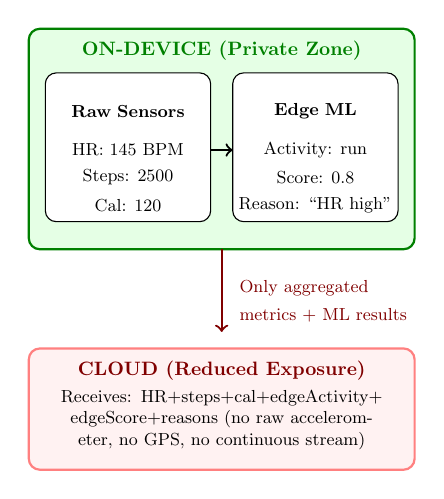
\begin{tikzpicture}[scale=0.7, every node/.style={scale=0.7}]
    % Device boundary
    \draw[fill=green!10, rounded corners, thick, draw=green!50!black] (0,4) rectangle (7,8);
    \node[font=\bfseries, green!50!black] at (3.5,7.6) {ON-DEVICE (Private Zone)};

    \draw[fill=white, rounded corners] (0.3,4.5) rectangle (3.3,7.2);
    \node[font=\small, text width=2.5cm, align=center] at (1.8,6.5) {\textbf{Raw Sensors}};
    \node[font=\small] at (1.8,5.8) {HR: 145 BPM};
    \node[font=\small] at (1.8,5.3) {Steps: 2500};
    \node[font=\small] at (1.8,4.8) {Cal: 120};

    \draw[fill=white, rounded corners] (3.7,4.5) rectangle (6.7,7.2);
    \node[font=\small, text width=2.5cm, align=center] at (5.2,6.5) {\textbf{Edge ML}};
    \node[font=\small] at (5.2,5.8) {Activity: run};
    \node[font=\small] at (5.2,5.3) {Score: 0.8};
    \node[font=\small] at (5.2,4.8) {Reason: ``HR high''};

    \draw[->, thick] (3.3,5.8) -- (3.7,5.8);

    % Cloud boundary
    \draw[->, thick, red!50!black] (3.5,4) -- (3.5,2.5);
    \node[right, font=\small, red!50!black] at (3.7,3.3) {Only aggregated};
    \node[right, font=\small, red!50!black] at (3.7,2.8) {metrics + ML results};

    \draw[fill=red!5, rounded corners, thick, draw=red!50] (0,0) rectangle (7,2.2);
    \node[font=\bfseries, red!50!black] at (3.5,1.8) {CLOUD (Reduced Exposure)};
    \node[font=\small, text width=6cm, align=center] at (3.5,0.9) {Receives: HR+steps+cal+edgeActivity+ edgeScore+reasons (no raw accelerometer, no GPS, no continuous stream)};
\end{tikzpicture}
\caption{Edge-first privacy architecture: raw sensor data stays on-device.}
\label{fig:privacy_arch}
\end{figure}

\subsection{Data Minimization Analysis}

\begin{table}[H]
\centering
\caption{Data Transmitted vs. Data Retained On-Device}
\label{tab:data_min}
\begin{tabular}{lcc}
\toprule
\textbf{Data Type} & \textbf{Stays On-Device} & \textbf{Sent to Cloud} \\
\midrule
Raw HR stream (30s) & Yes & No* \\
Step count & Yes & Periodic aggregate \\
Calories & Yes & Periodic aggregate \\
Edge activity & Yes & Yes (class label) \\
Edge anomaly score & Yes & Yes (0-1 float) \\
Anomaly reasons & Yes & Yes (text) \\
Accelerometer data & Yes (not collected) & No \\
GPS/Location & N/A (not collected) & No \\
User identity & Yes & userId only \\
\bottomrule
\end{tabular}
\end{table}

*Heart rate values are sent as periodic snapshots (every 15-60 min), not continuous streams.

\section{Security Controls}

\subsection{Authentication Layer}

\begin{table}[H]
\centering
\caption{API Security Configuration}
\label{tab:api_security}
\begin{tabular}{ll}
\toprule
\textbf{Control} & \textbf{Implementation} \\
\midrule
Transport & TLS 1.2+ (HTTPS-only) \\
Authentication & API Key (X-API-Key header) \\
Key Storage (Watch) & Android Keystore \\
Key Storage (Mobile) & Secure Storage \\
Key Rotation & Manual (deploy.sh) \\
Rate Limiting & API Gateway throttling \\
CORS & Not applicable (native apps) \\
\bottomrule
\end{tabular}
\end{table}

\subsection{Data-at-Rest Encryption}

\begin{table}[H]
\centering
\caption{Encryption Configuration}
\label{tab:encryption}
\begin{tabular}{llll}
\toprule
\textbf{Storage} & \textbf{Encryption} & \textbf{Key Mgmt} & \textbf{Standard} \\
\midrule
DynamoDB & Server-side & AWS KMS & AES-256 \\
S3 (models) & Bucket-level & AWS KMS & AES-256 \\
Room DB & SQLCipher* & App-level & AES-256 \\
AsyncStorage & Platform & OS Keychain & Varies \\
\bottomrule
\end{tabular}
\end{table}
*SQLCipher recommended but not yet implemented.

\subsection{IAM Access Control}

\begin{table}[H]
\centering
\caption{Lambda IAM Permissions (Least Privilege)}
\label{tab:iam}
\begin{tabular}{lp{4.5cm}}
\toprule
\textbf{Lambda Function} & \textbf{Permissions Granted} \\
\midrule
HealthDataIngestion & DynamoDB:PutItem, DynamoDB:GetItem, Lambda:InvokeFunction, SNS:Publish \\
HealthAnomalyInference & S3:GetObject, DynamoDB:Query, DynamoDB:UpdateItem, SNS:Publish \\
HealthSnsToExpo & DynamoDB:Query (tokens only) \\
HealthReadMetrics & DynamoDB:Query (read-only) \\
\bottomrule
\end{tabular}
\end{table}

\section{Regulatory Compliance Analysis}

\begin{table}[H]
\centering
\caption{Regulatory Compliance Status}
\label{tab:compliance}
\begin{tabular}{p{1.5cm}p{2cm}p{1.2cm}p{2cm}}
\toprule
\textbf{Regulation} & \textbf{Requirement} & \textbf{Status} & \textbf{Gap} \\
\midrule
HIPAA & Encryption at rest & Met & None \\
HIPAA & Access controls & Met & Audit logs \\
HIPAA & BAA with AWS & Partial & Needs formal \\
GDPR & Data minimization & Met & None \\
GDPR & Right to erasure & Partial & No API yet \\
GDPR & Consent mgmt & Partial & No UI yet \\
DPDPA & Data localization & Met & ap-south-2 \\
DPDPA & Purpose limitation & Met & None \\
\bottomrule
\end{tabular}
\end{table}

\section{Privacy Risk Assessment}

\begin{figure}[H]
\centering
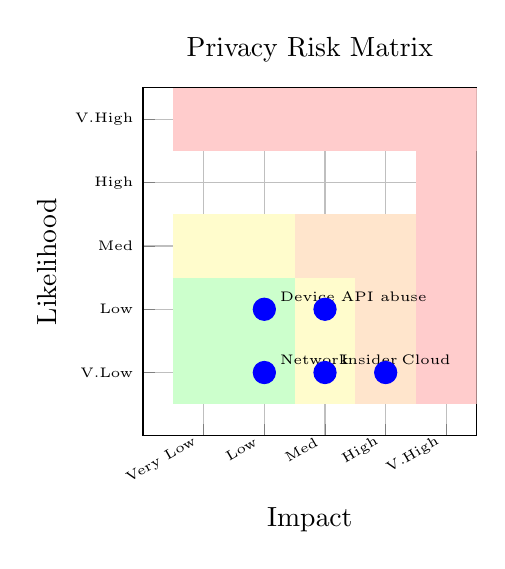
\begin{tikzpicture}
\begin{axis}[
    xlabel={Impact},
    ylabel={Likelihood},
    xmin=0, xmax=5.5,
    ymin=0, ymax=5.5,
    grid=major,
    width=0.48\textwidth,
    height=6cm,
    title={Privacy Risk Matrix},
    xtick={1,2,3,4,5},
    ytick={1,2,3,4,5},
    xticklabels={Very Low, Low, Med, High, V.High},
    yticklabels={V.Low, Low, Med, High, V.High},
    x tick label style={font=\tiny, rotate=30, anchor=east},
    y tick label style={font=\tiny},
]
% Fill risk zones
\fill[green!20] (0.5,0.5) rectangle (2.5,2.5);
\fill[yellow!20] (2.5,0.5) rectangle (3.5,2.5);
\fill[yellow!20] (0.5,2.5) rectangle (2.5,3.5);
\fill[orange!20] (2.5,2.5) rectangle (4.5,3.5);
\fill[orange!20] (3.5,0.5) rectangle (4.5,2.5);
\fill[red!20] (4.5,0.5) rectangle (5.5,5.5);
\fill[red!20] (0.5,4.5) rectangle (5.5,5.5);

\addplot[only marks, mark=*, mark size=4pt, blue] coordinates {
    (2, 1) % network eavesdropping (TLS mitigates)
    (4, 1) % cloud breach (encryption mitigates)
    (3, 2) % API abuse
    (2, 2) % device theft
    (3, 1) % insider threat
};
\node[font=\tiny, anchor=west] at (2.1, 1.2) {Network};
\node[font=\tiny, anchor=west] at (4.1, 1.2) {Cloud};
\node[font=\tiny, anchor=west] at (3.1, 2.2) {API abuse};
\node[font=\tiny, anchor=west] at (2.1, 2.2) {Device};
\node[font=\tiny, anchor=west] at (3.1, 1.2) {Insider};
\end{axis}
\end{tikzpicture}
\caption{Privacy risk matrix showing residual risk after controls.}
\label{fig:risk_matrix}
\end{figure}

\section{Privacy Comparison with Commercial Systems}

\begin{table}[H]
\centering
\caption{Privacy Comparison}
\label{tab:privacy_comparison}
\begin{tabular}{lcccc}
\toprule
\textbf{Privacy Feature} & \textbf{Apple} & \textbf{Fitbit} & \textbf{Samsung} & \textbf{Ours} \\
\midrule
Edge processing & Partial & No & Partial & \textbf{Yes} \\
Data minimization & Med & Low & Med & \textbf{High} \\
Open-source & No & No & No & \textbf{Yes} \\
Self-hostable & No & No & No & \textbf{Yes} \\
Auditability & Low & Low & Low & \textbf{Full} \\
Data ownership & Vendor & Vendor & Vendor & \textbf{User} \\
Regulatory compliance & High & Med & Med & \textbf{WIP} \\
\bottomrule
\end{tabular}
\end{table}

\section{Proposed Enhancements}

\subsection{End-to-End Encryption}
Implement application-level encryption using AES-256-GCM before transmission, ensuring data is encrypted even in the unlikely event of TLS compromise.

\subsection{Differential Privacy}
Apply $(\epsilon, \delta)$-differential privacy to aggregated statistics:
\begin{equation}
\tilde{f}(D) = f(D) + \text{Lap}\left(\frac{\Delta f}{\epsilon}\right)
\end{equation}

\subsection{Federated Learning}
Train ML models collaboratively across devices without sharing raw data:
\begin{equation}
w_{t+1} = w_t - \eta \sum_{k=1}^{K} \frac{n_k}{n} \nabla L_k(w_t)
\end{equation}

where each device $k$ computes local gradients $\nabla L_k$ on its private data.

\section{Discussion}
The edge-first architecture significantly reduces the privacy attack surface compared to cloud-centric alternatives. By performing anomaly detection on-device, raw continuous sensor data never leaves the watch. Only periodic aggregated snapshots (every 15-60 minutes) are transmitted with ML-derived labels.

However, the system currently lacks several enterprise-grade security features: audit logging, key rotation automation, formal BAA with AWS, and user consent management UI. These represent priority areas for hardening before any clinical deployment.

\section{Conclusion}
Our hybrid edge-cloud architecture implements a privacy-preserving health monitoring system through edge-first ML processing, data minimization, and layered security controls. The system reduces data exposure compared to commercial alternatives while maintaining detection accuracy through cloud-enhanced inference. Remaining gaps (audit logging, consent UI, end-to-end encryption) are identified for future implementation. We recommend the edge-first paradigm as a design pattern for privacy-sensitive wearable health applications.

\begin{thebibliography}{00}
\bibitem{hipaa} U.S. Department of HHS, ``HIPAA security rule,'' \textit{Federal Register}, 2003.
\bibitem{gdpr} European Parliament, ``General Data Protection Regulation (GDPR),'' \textit{EU Regulation 2016/679}, 2016.
\bibitem{dpdpa} Government of India, ``Digital Personal Data Protection Act,'' 2023.
\bibitem{dp_survey} C. Dwork and A. Roth, ``The algorithmic foundations of differential privacy,'' \textit{Foundations and Trends in TCS}, vol. 9, no. 3--4, pp. 211--407, 2014.
\bibitem{federated} B. McMahan et al., ``Communication-efficient learning of deep networks from decentralized data,'' \textit{Proc. AISTATS}, pp. 1273--1282, 2017.
\end{thebibliography}

\end{document}
